\chapter{Evaluation}\label{C:evaluation}

\section{Objectives}
\begin{enumerate} \label{experiment_objectives}
	\item{Can collaborative filtering provide personalised recommendations to users for the use case of ``Find Good Items"?}
	\item{Are personalised recommendations superior in accuracy than non-personalised recommendations based on the baseline predictor (item popularity)?}
	\item{Does a hybrid CF approach provide more accurate recommendations to a SVD CF approach?}
	\item{Does an item-based SVD CF approach provide more accurate recommendations than a Hybrid CF approach?}
	\item{Do correlated recommendations using binary ratings (Like/Dislike) provide more accurate recommendations than non-correlated binary ratings?}
\end{enumerate}

The objectives of this report focus on providing a base recommendation system that is able to fulfill the overall goal of ``Find Good Items" specified in Section \ref{C:intro}. To demonstrate whether the goal has been achieved, item popularity is used as a baseline predictor, comparing CF approaches to the baseline predictor which provides non-personalised recommendations. Additional objectives focus on comparing variations of latent factor CF approaches to a hybrid CF approach presented in Section \ref{algorithms}. The main objectives of the experiment are to answer the questions in Section \ref{experiment_objectives} in regard to the goal of ``Find Good Items".

\section{User Study}

The goal of the experiment is to provide a base recommendation system that provides personalised food dish recommendations to users in regard to the ``Find Good Items" use case. Collaborative filtering (CF) heavily relies on user data to provide recommendations. To capture data, a survey was given to participants asking them to rate their food preferences, indicate their food intolerances, and rate food dishes using a Likert Scale Rating system that best reflected their opinion about food dishes. This data was used in an offline experiment to evaluate latent factor CF approaches and a hybrid CF approach. Binary recommendation accuracy metrics were used to evaluate the performance of the CF algorithms in regards to the goal of ``Find Good Items", consisting of the following: recommendation accuracy, precision, recall, area under the curve (the receiving operator curve), and precision at top N (10). 

Due to time constraints and requirement of real user data for CF evaluation, an online or user study was unable to be conducted. Therefore, an offline evaluation is done to determine a suitable CF model for further online and user evaluation. 

\subsection{Participants}

A total of 91 participants were involved in the experiment. The majority of participants were students studying at the school of Engineering and Computer Science (ECS) from Victoria University of Wellington (VUW). An estimated number of 55 students were from a first year COMP102 (ECS) lecture and tutorial. An estimated number of 10 participants were in their honours or masters year in ECS recruited from the Honours CO232 lab at VUW, and an estimated number of 20 participants were from a Summer of Tech event that was held at Kelburn Campus at VUW. The remaining participants were students from around the 200 level Cotton (ECS) labs from VUW. The data collected from participants were approved by the Human Ethics Committee (HEC), and can be seen in Appendix \ref{appendix:hec}.

The ages and gender of participants were not captured due to continual changes submitted in the HEC process. It is estimated the majority of participants are students in the age range of 17-24 since the majority were recruited from the School of Engineering and Computer Science at Victoria University. It is possible a small number of participants are under or over the age range of 17-24, and may not be students. In addition, it is likely there are more male participants than female participants due to the location of recruitment.

Participants were asked to fill out surveys capturing their food preferences, food intolerances, and their opinions about food dishes. Strict food preferences were presented to participants as seen in Figure \ref{fig:strict_prefs}. The data around the participants strict food preferences collected from the survey can be seen in Table \ref{table:food_participants}:

\begin{figure}
\centering
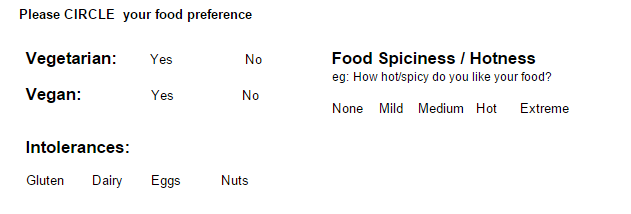
\includegraphics[scale=0.8]{images/strict_prefs.png}
\caption{Participants in the survey were asked to rate their food preferences and their opinions about food dishes based on using a Likert Scale rating system that best reflected how they felt about the item shown. The figure above illustrates the strict food preferences that are shown to participants.}
\label{fig:strict_prefs}
\end{figure}

\begin{table}[h!]
\centering
\begin{tabular}{|l|l|} 
 \hline
 \multicolumn{2}{|c|}{Percentage of Participants with Strict Food Preferences} \\
    \hline
    \hline
    Participants & Percentage \\
     \hline\hline
     Vegetarian & 7\%\\ [0.5ex] 
     \hline
     Vegan & 5\% \\
     \hline
     Gluten Intolerant & 8\% \\
    \hline
     Diary Intolerant & 5\% \\
     \hline
     Nuts Intolerant & 0\% \\
     \hline
     Egg Intolerant & 0\% \\
     \hline
     Other Intolerance & 0\% \\
     \hline
\end{tabular}
\caption{Percentage of participants in the whole dataset that have strict food preferences.}
\label{table:food_participants}
\end{table}

\subsection{Survey}

Quantitative data about user food ratings were collected from participants in a survey. Participants were asked to rate their food preferences, their food intolerances, and their opinion about food dishes from the following Likert Scale rating system: Hate, Dislike, Neutral, Like, and Love. Food preferences refer to preferences such as meat, pastry, soup, noodles etc. Food intolerances refer to intolerance to gluten, dairy, nuts etc. Food dishes refer to a variety of food that is ready to eat such as Thai Green Chicken Curry, Fried Chicken, Butter Bean Salad and so fourth. Participants were asked to circle the rating that best reflected their opinion based on using Likert Scale ratings as seen in Figure \ref{fig:survey}.

\begin{figure}
\centering
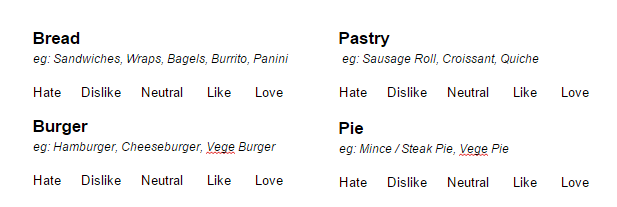
\includegraphics[scale=0.8]{images/survey_preferences.png}
\caption{Participants in the survey were asked to rate their food preferences based on using a Likert Scale rating system that best reflected how they felt about the food preference shown. The figure above illustrates a 4 food preferences that are shown to participants.}
\label{fig:survey}
\end{figure}

\begin{figure}
\centering
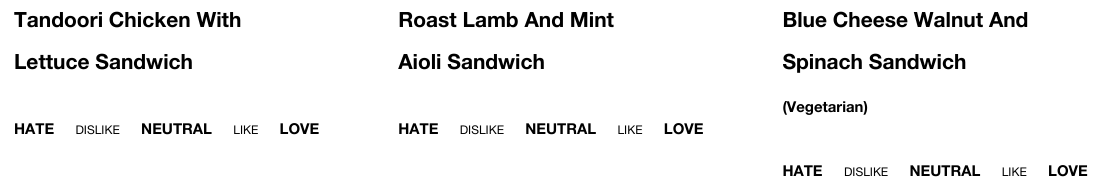
\includegraphics[scale=0.5]{images/survey_foods.png}
\caption{Participants in the survey were asked to rate food dishes based on using a Likert Scale rating system that best reflected how they felt about the food dish shown. The figure above illustrates a 3 food dishes that are shown to participants.}
\label{fig:survey_food}
\end{figure}

The survey contained 100 food dishes, 21 food preferences, and 5 food intolerances for participants to rate. The full list can be found in Appendix \ref{appendix:survey}. Any unrated items were classified as Neutral ratings inferring participants had no opinion about the food dish at the current time of rating or that they had not tried the food dish before. The survey was grouped into categories for participants to filter through the food dishes efficiently. All participants were shown the same food dishes but the ordering of the categories were randomised to help mitigate biases such as participants rating only the first items they see and so fourth. All food dishes were captured from food vendors in the facility of Kelburn campus at Victoria University of Wellington. Only the title of the food dishes were shown to participants, other information such as images were explicitly excluded. This was to prevent biases around the imagery, the price of the dish, the food vendor of where the food can be purchased etc, since these factors can influence the way participants rate the dishes (especially if majority of participants are students). For example, a participant could like a food dish such as a Butter Chicken Pie from a specific food vendor, but hate it from another food vendor. The image of a food dish may also influence the way participants rate a dish, therefore, excluding this information enables the representation of the participants general food preferences to be captured. A variety of food dishes have also been included in the survey to ensure there are options for all users such as users with intolerances, and users that are vegans or vegetarians. 

Despite this, mistakes were made in the creation of the survey. A small number of food dishes have been incorrectly labelled ``vegetarian" such as Chicken Curry \& Feta, and Chicken Fried Rice. The survey ``Intolerances" section should have also contained the following options: Other, N/A. In addition, the survey should have asked users to only rate food dishes they have explicitly tried before, rather than rating food dishes that best reflected their opinion. The latter is ambiguous since participants may rate food dishes based on dishes they want to try. This is not an accurate representation of actual food preference from the users, which may influence results in the experiment. Another mistake was raised by a vegetarian participant who had notified on the survey that their were no vegetarian dishes in the sushi category. This mistake was based on the choice of food dishes in the survey, since there are 100 food dishes, the length of the survey may cause fatigue in participants and it can be difficult defining a set length.   

The following section details the data collected from the survey. 

\section{Dataset} \label{dataset}

In the context of this project, a rating is referred to as a set of $(u, i, r)$ triplets, where a user $u$ has given a rating $r$ on an item $i$. 
The ratings collected from the survey consist of the following rating values: Hate (-1.0), Dislike (-0.5), Neutral (0.0), Like (0.5), and Love (1.0). Since Binary rating data is only used in the recommender system, Like and Love ratings are considered to be both positive ratings and can be considered as one event, in this case, a Like rating (Referring to any positive rating). Dislike and Hate ratings are also considered as one event and are combined to represent a Dislike event (Referring to any negative rating). Although this project focuses on Binary rating data only, the rationale of collecting multiple rating events was for backup purposes or future evaluation, if binary rating events are found to provide insufficient information to the recommender system. 

The original data collected from the survey consists of the following:
The dataset can be seen in the following table \ref{table:original_dataset}:

\begin{table}[h!]
\centering
\begin{tabular}{|l|l|} 
 \hline
 \multicolumn{2}{|c|}{Original Dataset} \\
     \hline\hline
     Name & Number\\ [0.5ex] 
     \hline
     Users & 91 \\
     \hline
     Food Dishes & 100 \\
     \hline
     Available Food Preferences & 21 \\ 
     \hline
     Available Food Intolerances & 5 \\ 
     \hline
     Ratings & 9100 \\
     \hline
     Like Ratings (Positive) & 4207 \\
     \hline
     Dislike Ratings (Negative) & 1638 \\ [1ex] 
     \hline
     Food Preference Ratings (Negative) & 813 \\ [1ex]
     \hline
\end{tabular}
\caption{A table showing the original dataset collected from the survey.}
\label{table:original_dataset}
\end{table}

% 
% The sparsity of a rating dataset is defined as the density of the vacancies in
% the user-item rating matrix, as in equation 2.1.
% sparsity = 1 −
% # ratings
% # users × # items
% (2.1)
% Because most users would have only rated a very small portion of the
% items, most recommendation datasets have very high sparsity, with sparsity
% as high as 0.95 considered normal [129].3 For this reason, in the field of
% recommender systems, the term “sparse” only refers to the extreme cases
% where the sparsity of the dataset is higher than 0.99. Such extreme sparsity normally occurs when new recommender systems are first established, or
% in datasets where the number of users is small relative to the volume of
% information in the system due to either a large number of items or regular
% updates of the item pool or both.

\subsection{Data Cleansing}

Collaborative filtering algorithms depend heavily on user data to give personalised recommendations. Therefore, the validity of user data can influence how collaborative filtering algorithms perform on the data. To mitigate this, data cleansing is conducted, removing any information from users that provided dubious answers found in the survey. Many answers from the survey contained conflicting ratings from participants, examples were participants who indicated they were vegetarians, but had rated meat dishes positively. These users along with their rating information were removed and were apparent since authentic vegetarian participants rated ``Hate" for every food dish containing meat. A subset of users provided answers to the survey that were difficult to decipher, for example, participants indicated intolerances to gluten but had then positively rated food dishes containing gluten. This could mean several participants may have differing levels of tolerance to gluten, or perhaps expressed they enjoy the gluten free version of the food dish and so fourth. Therefore, any user data that was ambiguous was not removed from the dataset to maintain validity. In addition, cases where participants did not finish rating all items were preserved. Table \ref{table:cleansed_dataset} demonstrates the data after it had been cleansed:

\begin{table}[h!]
\centering
\begin{tabular}{|l|l|} 
 \hline
 \multicolumn{2}{|c|}{Cleansed Dataset} \\
     \hline\hline
     Name & Number\\ [0.5ex] 
     \hline
     Users & 80 \\
     \hline
     Food Dishes & 100 \\
     \hline
     Available Food Preferences & 21 \\ 
     \hline
     Available Food Intolerances & 5 \\ 
     \hline
     Total Ratings & 8000 \\
     \hline
     Like Ratings (Positive) & 3937 \\
     \hline
     Dislike Ratings (Negative) & 1440 \\ [1ex] 
     \hline
     Neutral Ratings (Default) & 2620 \\ [1ex] 
     \hline
     Food Preference Ratings & 613 \\ [1ex] 
     \hline
\end{tabular}
\caption{A table showing the cleansed dataset where all the users that provided contradictory or invalid answers to the questions, had been removed.}
\label{table:cleansed_dataset}
\end{table}

\section{Experimental Background}

In this experiment, an offline evaluation is performed to evaluate the performance of CF algorithms based on the goal of ``Find Good Items". The method used consists of partitioning the dataset, tuning parameters from the recommendation system, and evaluating the performance of CF algorithms using binary recommendation accuracy metrics \cite{zhang}. 

\subsubsection{Data Partitioning} \label{partitioning}

Standard offline evaluations consist of partitioning a dataset into a training set and a test set, containing rating triplets described in Section \ref{dataset}. The training set is used by the recommendation system to learn the food preferences of users, providing recommendations based on predictions made about what the user likes from learning their preferences. Since the training set and test set are separate datasets, all rating triplets in the test set are unseen to the recommendation system and have not been learnt by the recommendation system during the training process. Therefore the ratings inside the test set is used to evaluate the performance of the recommendation system by checking whether the user has liked or disliked items recommended by the system. In addition, this is used to evaluate the generalisability of the recommendation system, giving insight to how well it may perform in a real scenario since the model has not seen the instances from the test data. 

In cases where the recommendation system contains tunable parameters, the dataset is partitioned into three datasets: a training set, a testing set, and a validation set. In the context of recommender systems, the validation set is used to find the optimal parameter settings but can also be used to reduce overfitting of the data, providing insight to the generalisability of the model. The validation set is used to evaluate the performance of the parameters, after the model has learnt on the training set. After the optimal parameters are found from the validation set, the test set is then used to evaluate the final performance of the recommender system. This prevents biases since the optimal parameters have not been learnt using the test set. Partitioning protocols and techniques exist to determine the partitioning of the datasets. This project uses the \textit{skip-every-nth protocol} which is specifically designed for recommender systems \cite{zhang}.

The \textit{skip every nth protocol} \cite{zhang} is used to partition the dataset into a training set and a test set. The \textit{skip-every-nth protocol} consists of randomising the ordering of users, and randomising the ratings within each user in a sequence that is contiguous to the user, aggregating the result in a list sequence \cite{zhang}. The protocol iterates through this list of user ratings assigning every \textit{nth} rating to the test set, the remaining ratings are assigned to the training set. The \textit{skip-every-nth protocol} ensures that ``the sparsity of the training dataset is minimally disturbed, and guarantees a (n - 1):1 size ratio between training and test data for all users up to decimal rounding" \cite{zhang}. However, since the \textit{nth} value affects the user ratings that are involved in the test set, this means users with few ratings may not be in the test set since their ratings may be skipped during the partitioning process. In these cases, evaluation is done \textit{n} times with the same ordering, but offsetting the partitioning each run by 1. This ensures that every user rating is used exactly once in the test set \cite{zhang}. 

The experiments in this report use the \textit{skip-every-10th protocol} to the dataset into a training set and the test set for final evaluation of the recommender system.

\subsubsection{Parameter Tuning}

Standard CF latent factor models have several parameters influencing the accuracy of recommendations, therefore, tuning parameters should be performed for optimal performance. Parameter tuning is typically performed using a training set and a validation set previously described in Section \ref{partitioning}. However, a validation set is not required as K-fold cross validation can be performed to find the optimal parameters of a model instead. 

K-fold cross validation \cite{kfold, campochiaro2009metrics} consists of partitioning a dataset into $k$ equal size folds (subsets). In the context of this project, the rating data contained within each fold is selected randomly. One fold from $k$ folds is selected as the validation set, the remaining folds $(k-1)$ are used as the training set. Evaluation metrics described in Section \ref{accuracy}, Section \ref{precision}, Section \ref{roc}, and Section \ref{auc} are then calculated. This is repeated $k$ times where each fold is used exactly once as a validation set. The evaluation results are then averaged, providing insight to how well the parameters perform for that run. In this project, K-fold validation is repeated multiple times, tuning the parameters in each run to find the optimal parameters. The optimal parameters found from multiple runs are then used for the final evaluation of the recommender system using the test set.

The advantage of K-fold cross validation is that every rating point is used exactly once in the validation set, and used in a training set $k-1$ times \cite{kfold}. However, since K-fold cross validation performs evaluation $k$ times, it can be computationally expensive to run \cite{kfold}.

A standard 10-fold cross validation is used to determine the optimal parameters in our experiments. 10-fold cross validation is performed on the training set, and is not performed on the test set. In this way, the test set remains uncontaminated since the optimised parameters have not been learnt from any rating data from the test set, preventing bias.

\subsubsection{Recommendation Accuracy} \label{accuracy}

In the context of recommender systems, recommendation accuracy measures the performance of a recommender system based on how well the system can correctly distinguish whether a user will like an item or whether they will not. This is similar to the decision users make in a real world scenario where decisions are based on ``acceptance or rejection" of items from the recommendations given \cite{zhang}. Therefore, recommendation accuracy metrics are appropriate for the use case of ``Find Good Items" \cite{evaluation} as it can ``evaluate how well the system is at assisting the final decision of the user" \cite{zhang}. 

Since the goal of this project is to ``Find Good Items", recommendation accuracy is used as a primary metric in our experiments. Although recommendation accuracy can measure the good and bad items for each user, it can not measure how much a user will like a food dish, or how much a user will dislike a food dish. All recommended food dishes are predicted to be liked by the user, and all unrecommended food dishes are predicted to be disliked. This means recommendation accuracy is unable to determine the ranking of preference for recommendations given to users, not being guaranteed to see their top preference in the recommendations list based on $n$ items. 

For these reasons, recommendation accuracy is used with supporting metrics of precision (Section \ref{precision}), recall (Section \ref{precision}), precision at top $N$ (Section \ref{precision}), and the area under the receiving operating characteristic curve (Section \ref{auc}). 

\subsubsection{Precision, Recall, and Precision at N} \label{precision}

There are four possible categories that binary recommendations from a recommender system can be classified as \cite{zhang}. These four possible categories can be seen in Table \ref{table:categories}. Recommended items preferred by users result in a True-Positive (TP). This represents an accurate result from the recommender system, since the user preferred the recommended item. Recommended items not preferred by users result in a False-Positive (FP). This represents an inaccurate result from the recommender system, since the user did not prefer the recommended item. Non-recommended items preferred by users result in a False-Negative (FN). This represents an inaccurate result from the recommender system, since the user preferred an item, but the item was not recommended by the recommender system. Non-recommended items not preferred by users result in a True-Negative (TN). This represents an accurate result from the recommender system, since the user did not prefer an item, and the item was not recommended by the recommender system.

\begin{table}[h!]
\centering
\begin{tabular}{|l|l|l|} 
     \hline
      & Recommended & Not Recommended \\ [0.5ex] 
     \hline
     Preferred & True-Positive (TP) & False-Negative (FN)\\
     \hline
     Not Preferred & False-Positive (FP) & True-Negative (TN) \\
     \hline
\end{tabular}
\caption{Categories recommendations}
\label{table:categories}
\end{table}

For binary ratings, precision and recall are often used as metrics. Precision measures the relevant recommendations (fidelity) to the user shown in Equation \ref{eq:precision}, whereas recall measures the relevant recommendations from the total preferred items (completeness) \ref{eq:precision}. 

Precision at $N$ uses Equation \ref{eq:precision} but only looks at the top $N$ recommendations list where $N$ is the number of recommended top items to the user. Precision at $N$ gives insight as to how many true liked items are in that list, and how many false liked items are not in the list. This can be used to measure the portion of relevant items that are recommended to users based on the top $N$ recommendation list, where only $N$ recommendations are shown.

\begin{equation} \label{eq:precision}
\centering
Precision = \frac{\#TP}{\#TP + \#FP}
\end{equation}

\begin{equation} \label{eq:recall}
\centering
Recall = \frac{\#TP}{\#TP + \#FN}
\end{equation}

% Recall, in its purest sense, is almost always impractical to measure in a
% recommender system. In the pure sense, measuring recall requires knowing
% whether each item is relevant; for a movie recommender, this would involve
% asking many users to view all 5000 movies to measure how successfully we recommend
% each one to each user

% Perhaps a more appropriate way to approximate precision and recall would
% be to predict the top N items for which we have ratings. That is, we take a
% user’s ratings, split them into a training set and a test set, train the algorithm
% on the training set, then predict the top N items from that user’s test set. If we
% assume that the distribution of relevant items and nonrelevant items within
% the user’s test set is the same as the true distribution for the user across all
% items, then the precision and recall will be much closer approximations of the
% true precision and recall. This approach is taken in Basu et al. [1998].
% In information retrieval, precision and recall can be linked to probabilities
% that directly affect the user. If an algorithm has a measured precision of 70%,
% then the user can expect that, on average, 7 out of every 10 documents returned
% to the user will be relevant. Users can more intuitively comprehend the meaning
% of a 10\% difference in precision than they can a 0.5-point difference in mean
% absolute error

% One of the primary challenges to using precision and recall to compare different
% algorithms is that precision and recall must be considered together to
% evaluate completely the performance of an algorithm.

% Precision alone at a single search length or a single recall level can be appropriate
% if the user does not need a complete list of all potentially relevant
% items, such as in the Find Good Items task. If the task is to find all relevant
% items in an area, then recall becomes important as well. However, the search
% length at which precision is measured should be appropriate for the user task
% and content domain.

\subsubsection{ROC Curves and Area Under The Curve} \label{roc} \label{auc}
In the context of this project, Receiver Operating Characteristic (ROC) curves can be used to visualise all the trade-offs between the True-Positive Rate, and the False-Positive Rate of a recommender system. The ROC cruve is computed by using all possible thresholds on a graph , and visualising the trade-off between the True-Positive Rate and the False-Positive Rate, displaying how well a model is able to distinguish recommendations that the users find relevant. The True Positive (TP) rate which is the y-axis, shows the sensitivity of the model. This means that it shows the fraction in which liked items by specific users are correctly recommended to the users. The False Positive (FP) rate which is the x-axis, shows the fraction in which disliked items by specific users are incorrectly recommended as items they would like. The Area Under The Curve (AUC) is a measure that can determine how good the recommender system is over all the thresholds, where a AUC of 1.0 specifies a recommendation system that recommends items perfectly to users. 

\section{Experimental Design}

\subsection{Setup/Tools}
The following equipment and tools were used to run the experiment:
\begin{itemize}
	\item{Intel(R) Core(TM) i7-4770 CPU @ 3.40GHz}
	\item{NVIDIA Quadro K620 GPU 2GB DDR3}
	\item{8GB DD3 RAM}
	\item{Arch 64bit GNU/Linux Operating System}
	\item{The programming language Ruby for the application WOTM}
	\item{PredictionIO 9.4 using HBase for the event server, and running on Apache Spark}
	\item{PredictionIO Engine written in Scala using Apache MLLib}
\end{itemize}

\subsection{Method} \label{method}

\begin{figure}
\centering
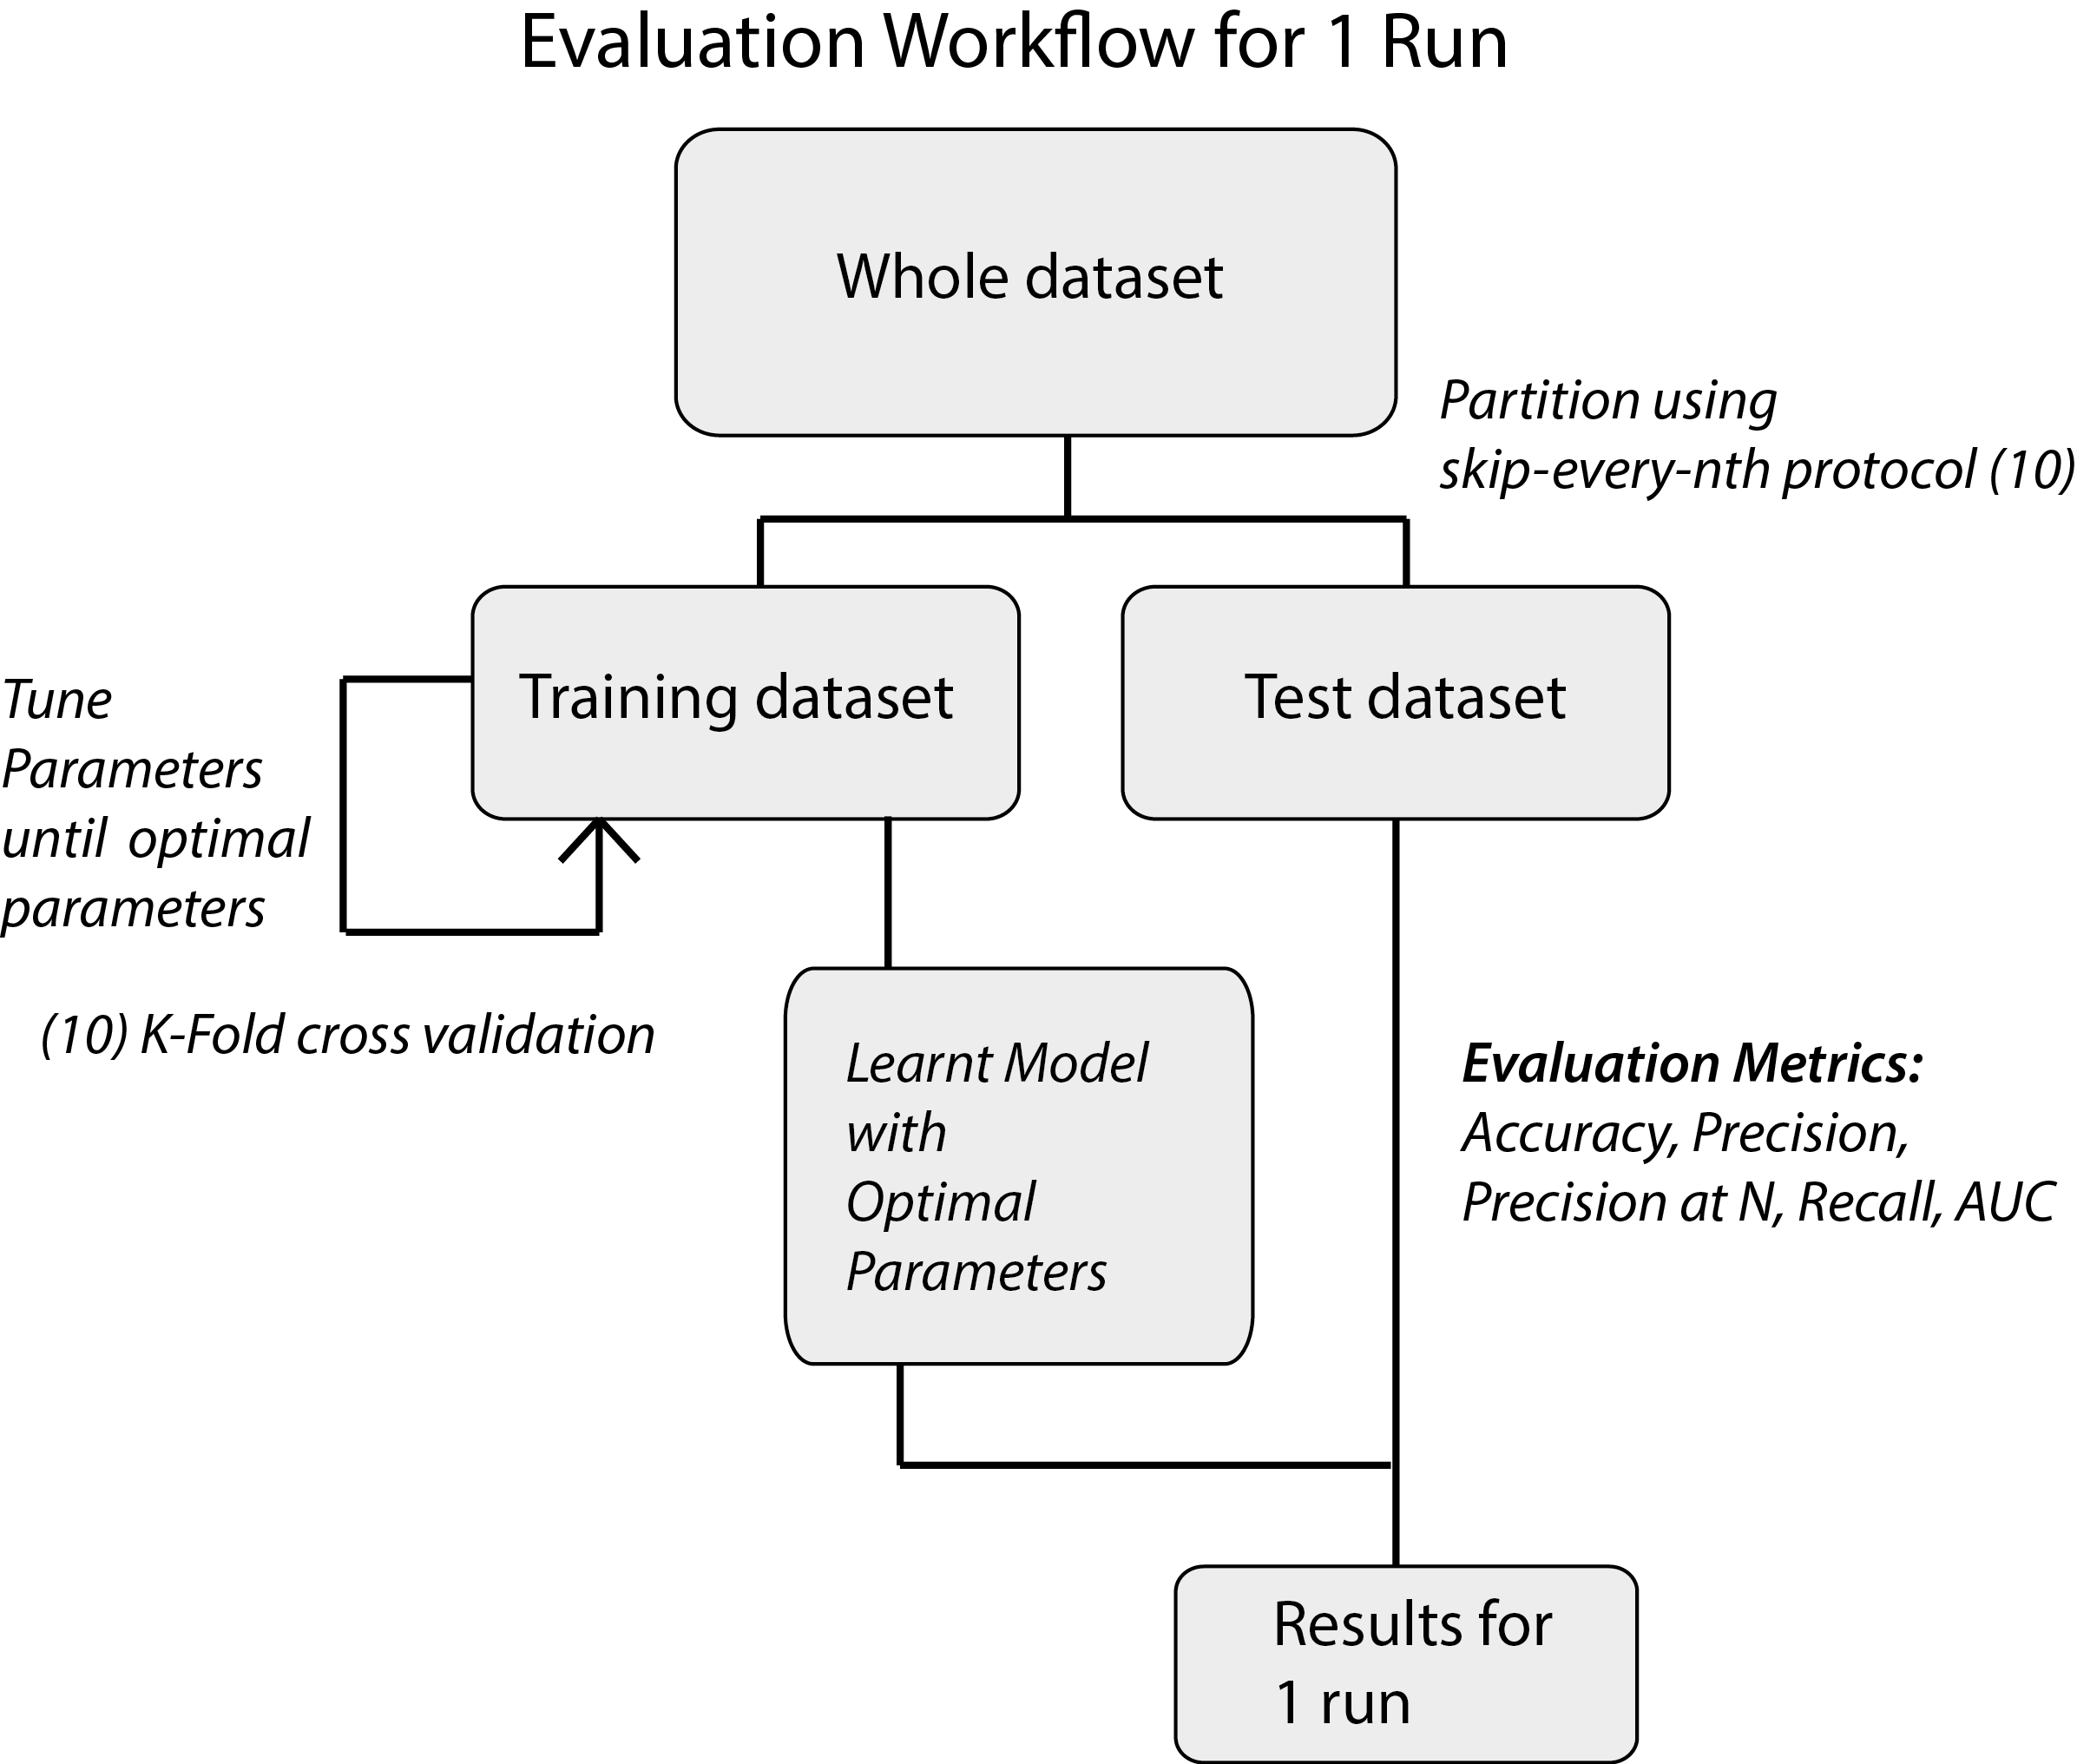
\includegraphics[scale=0.7]{recent_images/evaluation_workflow.png}
\caption{Evaluation for 1 run. Multiple runs are computed, and the results are averaged.}
\label{fig:evaluation_workflow}
\end{figure}

An offline study is evaluated using the dataset collected from the user study \ref{fig:evaluation_workflow}. The evaluation process can be shown in Figure \ref{fig:evaluation_workflow}. \textit{Skip-every-10th protocol} is used as the partitioning strategy to create a training set and a test set. The test set is used for the final evaluation of the learnt model when the optimal parameters have been found. 10-fold cross validation is performed on the training set multiple times with different parameters for the model until the optimal parameters are discovered. Since cross-validation uses each subset as validation data, we retrain the model on the whole training set data with the optimal parameters obtained from the k-fold validation. Using this model, evaluation is done on the test set computing the recommendation accuracy, the precision, the recall, and the precision at N (10). The results are then averaged over 30 runs. This method means that the parameters are not finalized since different optimal parameters are found every run. 

Therefore, another method is used to finalize the parameters. This method consists of doing the same above, but instead of doing the optimal parameters for every run, we use the same optimal parameters from the first run to test the remaining 29 runs. In this way, the parameters are finalized but the results of the data are contaminated since the learnt model in the remaining runs may have been trained on data from the test dataset from the first run.  

\section{Experimental Results}

In this section we present the results of the experiments described in Section \ref{method}. We will focus on comparing the hybrid CF approach to the Single SVD CF approach, demonstrating the use of food dish content used inside the hybrid CF technique is able to outperform the Single CF SVD approach. 


% This section also demonstrates the optimal parameters for the different approaches for further investigation in a commercial/real world environment.  

\begin{figure}[!tbp]
  \centering
  \begin{minipage}[b]{0.45\textwidth}
    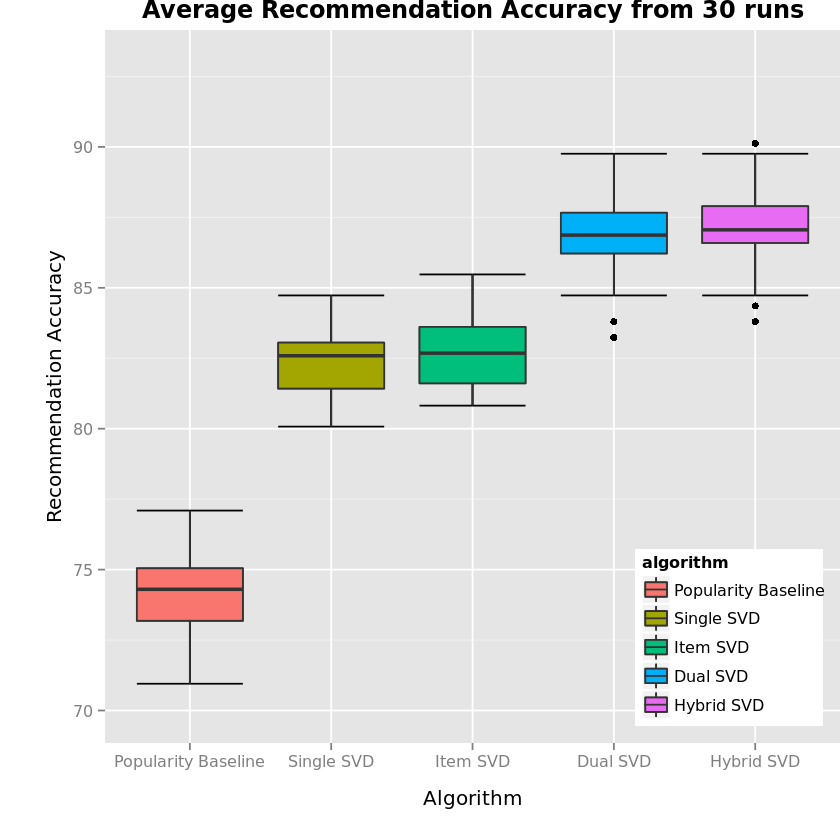
\includegraphics[width=\textwidth]{recent_images/accuracy.png}
    \caption{Average accuracy from 30 runs for different algorithms.}
    \label{fig:accuracy}
  \end{minipage}
  \hfill
  \begin{minipage}[b]{0.45\textwidth}
    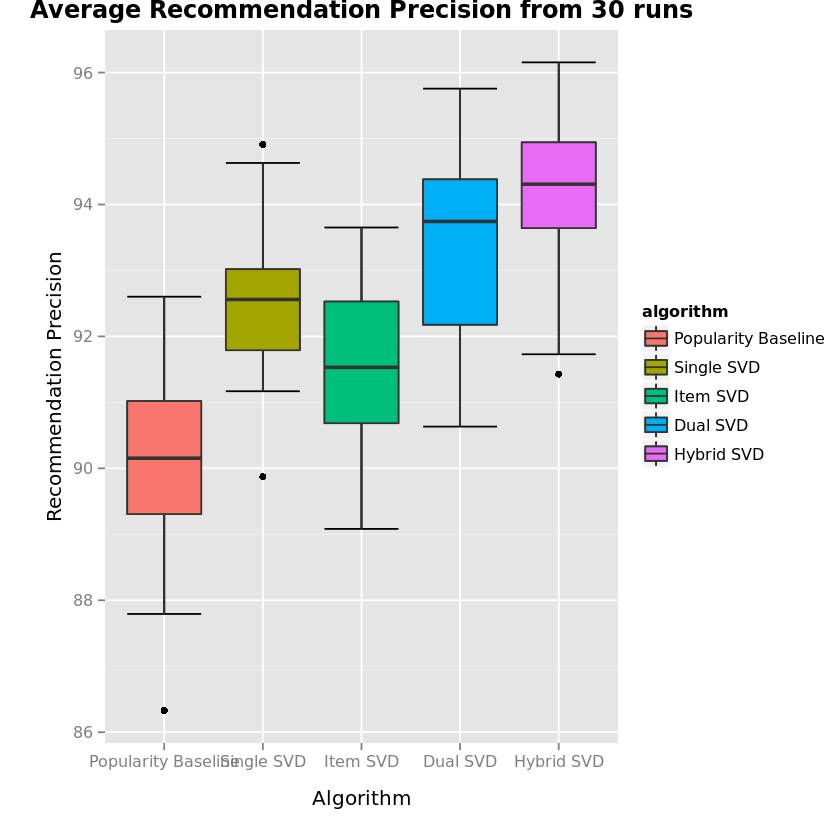
\includegraphics[width=\textwidth]{recent_images/precision.png}
    \caption{Average precision from 30 runs for different algorithms}
    \label{fig:precision}
  \end{minipage}
\centering
  \hfill
  \begin{minipage}[b]{0.45\textwidth}
    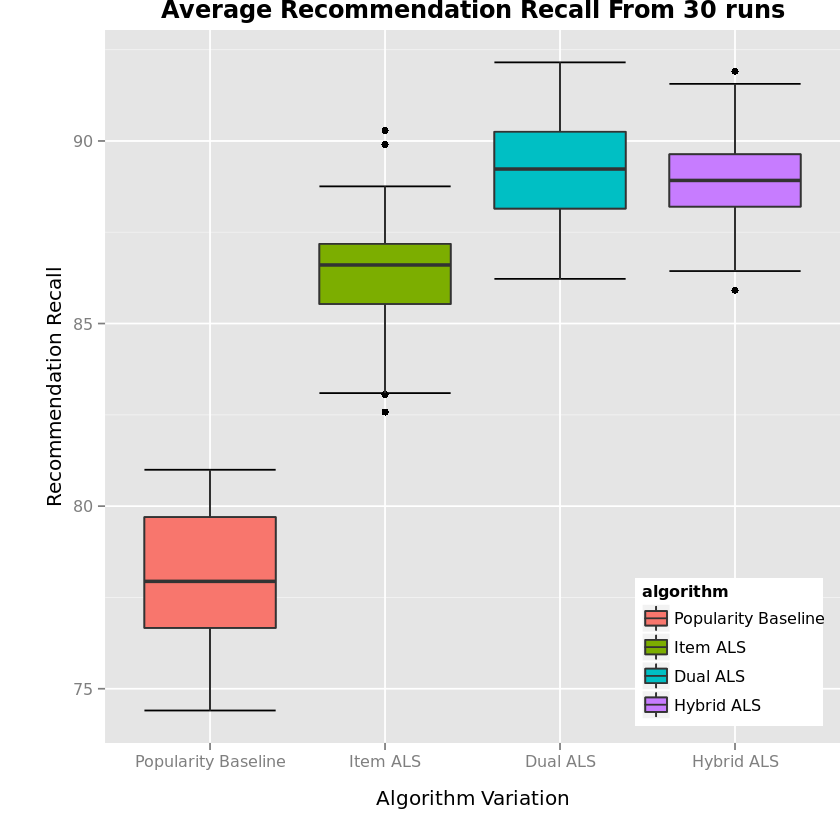
\includegraphics[width=\textwidth]{recent_images/recall.png}
    \caption{Average recall from 30 runs for different algorithms}
    \label{fig:recall}
  \end{minipage}
  \hfill
  \begin{minipage}[b]{0.45\textwidth}
    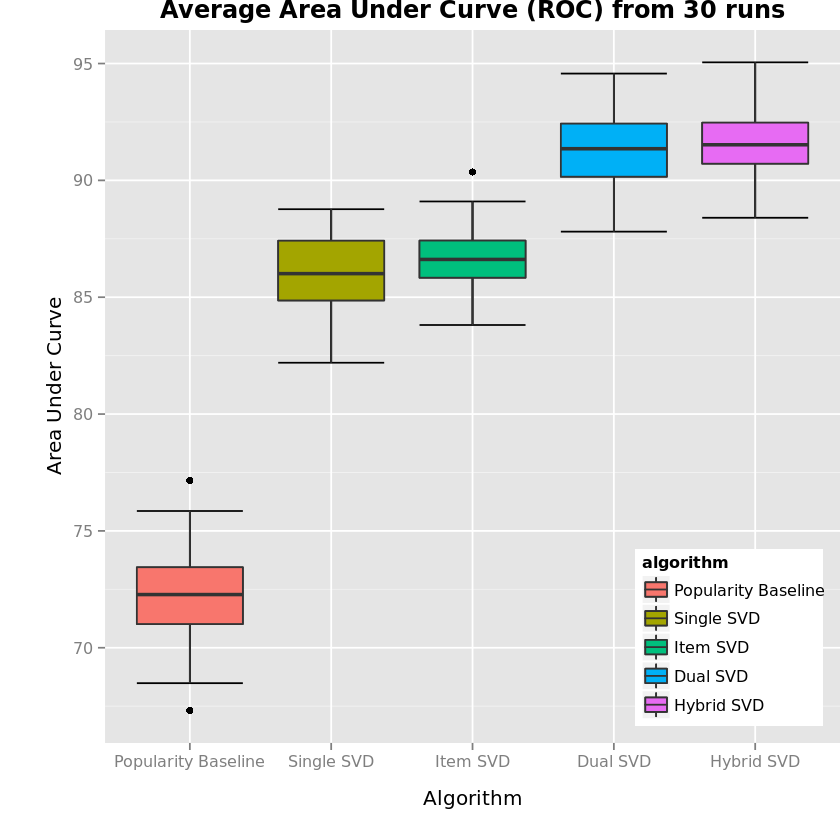
\includegraphics[width=\textwidth]{recent_images/auc.png}
    \caption{Average area under the roc curve for 30 runs over different algorithms}
    \label{fig:auc}
  \end{minipage}
\end{figure}

\begin{figure}
\centering
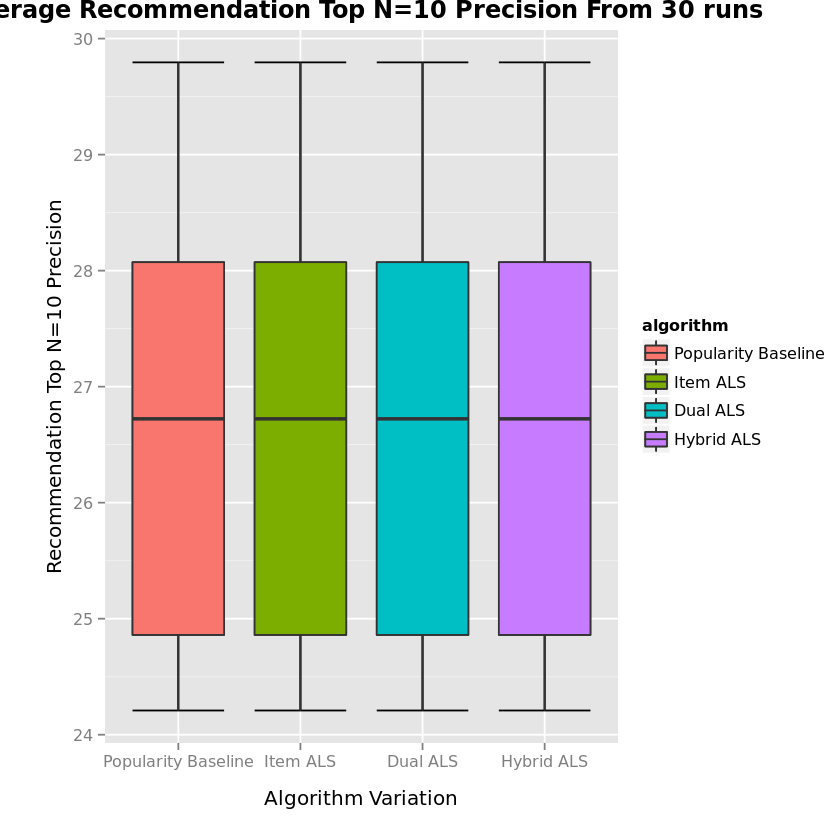
\includegraphics[scale=0.6]{recent_images/top_n.png}
\caption{Average precision at top n (10) for 30 runs over different algorithms}
\label{fig:top_n}
\end{figure}

\begin{figure}
\centering
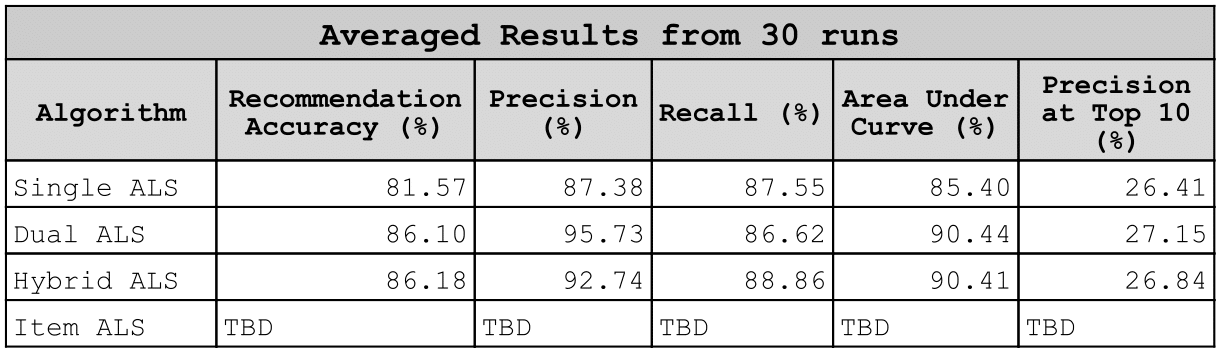
\includegraphics[scale=0.3]{images/results_tuning.png}
\caption{Averaged results ran 30 times with the same optimal parameters (contaminated).}
\label{fig:results}
\end{figure}

\subsection{Average Recommendation Accuracy}
Results are shown in \ref{fig:results} and \ref{fig:accuracy}. Recommendation accuracy is the most suitable for the use case of ``Find Good Items". From the results, the hybrid collaborative filtering seems to provide the highest accuracy in this case. The preferences from each user describing the attributes the user likes and dislikes, provides extra information to the recommender system, thus resulting in the higher accuracy. However, this information may not be available. The Hybrid CF approach was able to achieve an accuracy an 87.06 \%, where as the Dual SVD system achieved an 86.74\% accuracy. Although this is just a minor difference, the attributes of a food dish only contain three categories: meat type, food type, and cuisine type. These attributes provide extra information about the user, therefore provide higher accuracy. Although tagging of this information for each dish can be tedious, and is expected that errors may occur in labelling the data which may have affected the accuracy. In the other systems, Single SVD with an accuracy of 82\% was able to outperform the popularity baseline which had a accuracy of 73.84\%. This is expected since Single SVD is able to provide personalised recommendations whereas non-personalised are given by the popularity baseline. An unexpected case was the Item SVD was able to achieve an accuracy of 82.64\%, similar to that of the Single SVD 82.43\%. 

\subsection{Average Precision}

 From the results shown in \ref{fig:precision} and \ref{fig:results}, Dual SVD was able to achieve a higher precision (93.35\%) over the Single SVD (92.56\%) approach over multiple runs (30). This means the Dual SVD approach was able to more accurately recommend items the user preferred rather than the Single SVD. Since the average precision of the Single SVD is lower, it means that the recommender system recommended more items that users indicated they disliked (false positives). The lowest precision was the popularity baseline which provided non-personalised recommendations with a precision of 90\%. Item SVD achieved 91.64\% precision, where as the Hybrid CF approach achieved the highest precision of 94.19\%. 

\subsection{Average Recall}

From the results shown in \ref{fig:recall} and \ref{fig:results}, the system with the highest recall was the Dual SVD (89.03\%). The popularity baseline had the lowest recall of (72.21\%). The other system had the following recall rates: Single SVD (84.74\%), Item SVD (85.60\%), and Hybrid CF (87.06\%). Interestingly enough, the Hybrid CF performed better on all the other previous metrics (Accuracy and Precision), but had a lower recall rate than Dual SVD. Recall is closely related to Precision and their is usually a tradeoff between the two, since recall measures the amount of good items recommended from the total preference list of the user. This meant the Hybrid CF approach had recommended less of the total preferred items of users, than the Dual SVD approach. This might be the reason why the Hybrid approach had performed better than the Dual SVD in other metrics, since the sensitivity of the recommendations were higher than the Dual SVD system.

\subsection{Average AUC}

From the results shown in \ref{fig:auc} and \ref{fig:results}, the Hybrid CF approach achieved the highest AUC with 91.50\%. The Dual SVD achieved a similar result of 91.20\%. These results imply that the recommendations are good, since 90\% represents a good overall recommendation classifier holistically. Item SVD achieved a AUC of 86.67\%, Single SVD achieved a AUC of 84.76\%, and the popularity baseline achieved an AUC of 72.21\%. These indicate that the other systems performed fairly well. 

\subsection{Average Precision at top N (10)}

From the results shown in \ref{fig:top_n} and \ref{fig:results} all the systems have the same average precision of 27.08\% when 10 items are recommended to them. This means the same amount of preferred user items have appeared in the top 10 recommendations list. This is metric is suited towards providing insight about how users may perceive the recommendation algorithm in a real-world environment. For example, in an offline evaluation, users have already indicated the food dishes they have liked. If these food dishes are displayed at the top of the recommendations list, then it may establish trust between the user and the recommender system. 

\subsection{Experimental Conclusions}

In terms of the case of ``Find Good Items", all systems were able to achieve the goal, as they all provided personalised recommendations that performed better than non-personalised recommendations based on item popularity. In particular, the Hybrid CF approach was able to provide personalised recommendations at an accuracy of 87.06\%, outperforming the popularity baseline which provided non-personalised recommendations at an accuracy of 73.84\%. This fulfills the objectives 1 and 2 in \ref{experiment_objectives}. 

In terms of objective 3 in \ref{experiment_objectives}, the Item SVD achieved worse performance in all metrics compared to the Hybrid CF approach except precision at top n (10), where it achieved the same result. Item SVD achieved an accuracy of 82.65\%, being dominated by the Hybrid CF approach of 87.06\%. 

The Dual SVD was able to achieve an accuracy of 86.74\%, outperforming Single SVD which achieved 82.43\%. In addition, Dual SVD achieved better results in all other metrics except precision at top N (10), where the result was the same. Therefore, correlated recommendations based on binary ratings provide more accurate recommendations than non-correlated binary ratings. This claim backs up the claim that taking into the relationship between Like/Dislike of items provides overall better recommendations. 

Overall, a Hybrid CF approach was able to outperform every other system in terms of Accuracy, Precision, Area Under the Curve (ROC). Although the Dual SVD achieved a higher recall than the Hybrid, suggesting that more ``Good" items were recommended by the Dual SVD, the Dual SVD may not be better than the Hybrid CF approach since it recommended more items that users did not prefer. Ultimately, this is an important factor to consider, since recommending items users may not like, may cause distrust in the recommendations, leading to users less likely to use the system. 

\section{Limitations to Generalisability}

An offline experiment may not be enough as users may feel different in a real user evaluation. Therefore the following points indicate limitations to generalisability:
\begin{itemize}
	\item{Contradictions in the data and participation may lead to inaccurate recommendations}
	\item{Proportion of items and user may not be accurate in a real system}
	\item{Density and sparsity of the user-item rating matrix was densely filled.}
	\item{The survey questions need to ask the right questions}
\end{itemize}
Some people may have filled out dishes that they haven't tried before. This could affect the results because often what people do is different to what they think. 
There were cases where people filled out the form inaccurately, such that they chose random dishes. We know this because there are cases where someone states that they are “vegetarians” but then say they like “meat” etc.
Cleanse these cases to give better predictions

In addition, recommendation accuracy is identifying items that the user is already aware of, which makes it susceptible to biases involving overfitting and non-novel recommendations \cite{evaluation}. 



